\documentclass[11pt,a4paper]{article}

\usepackage[T1]{fontenc}
\usepackage[utf8]{inputenc}
\usepackage{lmodern}
\usepackage[margin=2.4cm]{geometry}
\usepackage{amsmath,amssymb,amsthm}
\usepackage{booktabs}
\usepackage{array}
\usepackage{xcolor}
\usepackage{fancyhdr}
\usepackage{titlesec}
\usepackage{hyperref}
\usepackage{tikz}
\usepackage{tcolorbox}
\usepackage{enumitem}
\usetikzlibrary{arrows.meta,positioning}

\definecolor{accent}{RGB}{30,74,118}
\definecolor{softbg}{RGB}{238,243,248}
\definecolor{rulegray}{RGB}{180,196,214}
\definecolor{codebg}{RGB}{244,247,250}

\hypersetup{
    colorlinks=true,
    linkcolor=accent,
    urlcolor=accent,
    citecolor=accent,
    pdftitle={Money-Laundering Ring Detection with Graph Algorithms},
    pdfauthor={Adityaa Saha, Debtanu Das, Jeeban Jyoti Patra, Shatadeep De}
}

\titleformat{\section}{\Large\bfseries\color{accent}}{\thesection}{0.8em}{}
\titleformat{\subsection}{\large\bfseries\color{accent}}{\thesubsection}{0.7em}{}

\pagestyle{fancy}
\fancyhf{}
\fancyhead[L]{\small\color{black!75}Money-Laundering Ring Detection}
\fancyhead[R]{\small\color{black!75}MFCS Group Project}
\fancyfoot[C]{\small\thepage}
\renewcommand{\headrulewidth}{0.4pt}
\renewcommand{\footrulewidth}{0pt}

\theoremstyle{definition}
\newtheorem{definition}{Definition}
\newtheorem{invariant}[definition]{Invariant}
\newtheorem{theorem}[definition]{Theorem}
\newtheorem{lemma}[definition]{Lemma}
\newtheorem{claim}[definition]{Claim}

\newtcolorbox{memberstrip}{
    colback=softbg,
    colframe=rulegray,
    boxrule=0.4pt,
    arc=2pt,
    left=8pt,right=8pt,top=5pt,bottom=5pt,
    before skip=4pt,after skip=10pt
}

\newtcolorbox{codebox}{
    colback=softbg,
    colframe=rulegray,
    boxrule=0.4pt,
    arc=2pt,
    left=8pt,right=8pt,top=6pt,bottom=6pt
}

\begin{document}

% ========================== TITLE PAGE ==========================
\begin{titlepage}
\thispagestyle{empty}
\centering
\vspace*{0.6cm}
{\large Indian Institute of Technology Bhubaneswar\\
School of Electrical and Computer Sciences\par}

\vspace{1.2cm}
{\color{accent}\rule{\linewidth}{1.2pt}}\\[0.7cm]
{\Huge\bfseries Money-Laundering Ring Detection\\[0.25cm] with Graph Algorithms\par}
\vspace{0.55cm}
{\color{accent}\rule{\linewidth}{1.2pt}}

\vspace{0.9cm}
{\large Project Report --- Mathematical Foundations of Computer Science\par}

\vspace{1.4cm}
\begin{tabular}{lll}
\toprule
\textbf{Member} & \textbf{Name} & \textbf{Assigned Module} \\
\midrule
Member 1 & Adityaa Saha & Ingestion, Graph Model \& Kosaraju SCC \\
Member 2 & Debtanu Das & Temporal Cycles \& Fan-Out / Fan-In \\
Member 3 & Jeeban Jyoti Patra & Pass-Through Chains, $k$-Core \& Greedy Peeling \\
Member 4 & Shatadeep De & Edmonds-Karp Max-Flow, Exact Densest Subgraph \& Evaluation \\
\bottomrule
\end{tabular}

\vspace{1.8cm}
\raggedright
\hspace*{1.2cm}%
\begin{tabular}{@{}ll@{}}
\textbf{Language} & C++17, standard library only \\
\textbf{Source}   & four files, one program: \texttt{src/ingest\_scc.cpp}, \\
                  & \texttt{src/cycles\_fan.cpp}, \texttt{src/chains\_peeling.cpp}, \\
                  & \texttt{src/exact\_eval.cpp} \\
\textbf{Dataset}  & IBM Synthetic AML (\texttt{data/HI-Small\_Trans.csv}, 5.08M transfers) \\
\textbf{Date}     & November 2026 \\
\end{tabular}

\vfill
\end{titlepage}

% ========================== ABSTRACT & TOC ==========================
\setcounter{page}{1}

\begin{center}
\textbf{Abstract}
\end{center}
\noindent
Money laundering hides illicit funds in ordinary payment traffic. It does so through a few recurring structures: money that travels in a \emph{cycle} back to its origin, one account that \emph{fans out} to or \emph{fans in} from many accounts within a short time, \emph{chains} of accounts that pass a slightly reduced amount onward, and tight groups of accounts that trade densely with each other. We model a transaction log as a directed temporal multigraph and detect each structure with a deterministic graph algorithm. There is no machine learning. Every detector comes with a formal definition, a correctness argument and a complexity bound. The detectors are Kosaraju's strongly connected components with a bounded-length temporal cycle search, a sliding-window fan detector, a longest-path dynamic program for layering chains, $k$-core decomposition with Charikar's greedy $\frac{1}{2}$-approximation, and an exact densest-subgraph algorithm via Goldberg's reduction to minimum cut. The whole system is 1\,392 lines of C++17 split evenly among four members. It passes 41 concrete self-checks covering edge cases and hand-computed textbook instances, and runs on the full 5.08-million-transfer IBM AML data set (\texttt{HI-Small\_Trans.csv}) in seconds.

\tableofcontents
\newpage

% ========================== SECTION 1 ==========================
\section{Introduction}

\subsection{Problem}
The input is a list of bank transfers, each with a timestamp, a sender account, a receiver account, an amount and (in labelled data) a flag saying whether it belongs to a laundering attempt. The goal is to flag the transfers that take part in laundering \emph{patterns}. The target data set is the IBM synthetic AML transaction data (\texttt{HI-Small\_Trans.csv}), which has eleven columns per row and a ground-truth ``Is Laundering'' label.

\subsection{Design principles}
\begin{itemize}[leftmargin=1.5em]
\item \textbf{Graph theory only.} Every detector is a deterministic graph algorithm with a theorem behind it. There are no trained models, neural networks or clustering heuristics.
\item \textbf{Each pattern is defined formally first.} The definition is then turned into an algorithm, the algorithm is proved correct, and only then is it coded.
\item \textbf{Tested before trusted.} Every algorithm is checked against an independent brute force on thousands of small random graphs, as well as on hand-made graphs whose answer is known.
\end{itemize}

\subsection{Division of work}
The work is split so that each member owns two algorithms, one major proof and one supporting invariant, and presents an equal share of the talk.

\medskip
\noindent
{\small
\setlength{\tabcolsep}{4.5pt}
\begin{tabular}{@{}cl>{\raggedright\arraybackslash}p{4.9cm}>{\raggedright\arraybackslash}p{4.9cm}r@{}}
\toprule
\textbf{Member} & \textbf{Name} & \textbf{Algorithms} & \textbf{Proofs} & \textbf{Lines} \\
\midrule
1 & Adityaa Saha & CSV ingestion and graph model; synthetic generator; Kosaraju SCC & Kosaraju correctness (Thm.~3); sorted adjacency (Inv.~2) & 413 \\
2 & Debtanu Das & Bounded temporal cycles; fan-out / fan-in & Cycle search exact (Thm.~6); sliding window (Claim~8) & 391 \\
3 & Jeeban Jyoti Patra & Pass-through chains; $k$-core and greedy peeling & $\frac{1}{2}$-approximation (Thm.~12); chain DP (Claim~10) & 464 \\
4 & Shatadeep De & Edmonds-Karp max flow; exact densest subgraph; evaluation harness; \texttt{main} & Min-cut reduction (Thm.~14, 15) & 286 + 226 \\
\bottomrule
\end{tabular}
}

% ========================== SECTION 2 ==========================
\section{Graph model and program structure}

\subsection{The transaction graph}
\begin{definition}[Transaction multigraph]
$G = (V, E)$ is a directed multigraph. $V$ is the set of accounts, identified by the string ``bank:account'' and numbered $0, \dots, n - 1$. Each transfer is an edge $e = (\text{tail}(e), \text{head}(e))$ with amount $a(e)$ (the \emph{Amount Paid} column) and timestamp $t(e)$ in seconds since 1970-01-01 UTC. Parallel edges are kept, because repeated transfers between the same pair carry information. Self loops are also kept and counted, and every detector skips them explicitly. The edges are indexed $0, \dots, m - 1$ in non-decreasing timestamp order.
\end{definition}

Each vertex $u$ stores two adjacency lists of edge indices: $\text{out}(u)$ and $\text{in}(u)$. Dense-subgraph detectors use the \emph{simple undirected projection} $H$, in which $\{u, v\}$ is an edge if and only if $u \ne v$ and at least one transfer goes between them in either direction. For $S \subseteq V(H)$, $E(S)$ is the set of edges with both ends in $S$, and the \emph{density} is $\rho(S) = |E(S)| / |S|$.

\subsection{One program in four files}
The project is a single program. The four files form an include chain, and the last file contains \texttt{main}:

\begin{center}
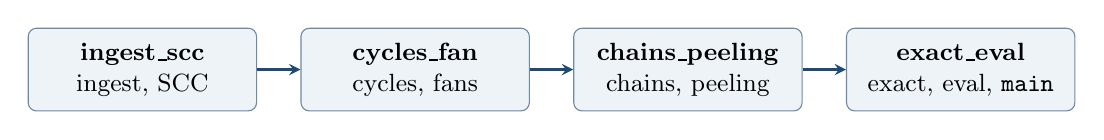
\begin{tikzpicture}[
    box/.style={draw=accent!65, fill=softbg, rounded corners=3pt, align=center, font=\small, minimum width=2.9cm, minimum height=1.05cm},
    arr/.style={->, >=stealth, thick, color=accent}
]
\node[box] (m1) {\textbf{ingest\_scc}\\ingest, SCC};
\node[box, right=0.55cm of m1] (m2) {\textbf{cycles\_fan}\\cycles, fans};
\node[box, right=0.55cm of m2] (m3) {\textbf{chains\_peeling}\\chains, peeling};
\node[box, right=0.55cm of m3] (m4) {\textbf{exact\_eval}\\exact, eval, \texttt{main}};
\draw[arr] (m1) -- (m2);
\draw[arr] (m2) -- (m3);
\draw[arr] (m3) -- (m4);
\end{tikzpicture}
\end{center}

Each file has include guards, and it defines its own \texttt{main} only when it is the file being compiled. As a result every member can build and test their part alone, and the full system builds with a single command:

\begin{codebox}
\small\ttfamily
clang++ -std=c++17 -O2 src/exact\_eval.cpp -o aml\\
./aml test \hspace{3.6cm}\# every member's self-tests\\
./aml generate data/synth.csv \hspace{1.35cm}\# labelled synthetic file\\
./aml detect \hspace{0.2cm} data/HI-Small\_Trans.csv \hspace{-0.05cm}\# one report section per member\\
./aml evaluate data/HI-Small\_Trans.csv \hspace{-0.05cm}\# precision / recall / timing tables
\end{codebox}

\noindent
The optional parameters, in order and with their defaults, are: cycle length $K = 6$, cycle window $W = 168\,\text{h}$, a safety cap of $10^6$ cycles, fan size $k = 5$, fan window $24\,\text{h}$, chain length $L = 3$, chain delay $D = 24\,\text{h}$ and chain tolerance $\varepsilon = 0.10$.

\newpage
% ========================== SECTION 3 ==========================
\section{Member 1 --- Ingestion and strongly connected components}

\begin{memberstrip}
\small\textbf{Member 1 --- Adityaa Saha} \hfill \texttt{src/ingest\_scc.cpp} \quad Graph, CSV loader, synthetic generator, Kosaraju SCC
\end{memberstrip}

\subsection{Ingestion}
The loader reads the eleven IBM columns. It parses timestamps such as \texttt{2022/09/01 00:20} with a hand-written days-from-civil routine, because \texttt{timegm} is not portable. Account names are interned to integers through a hash map. Malformed rows are skipped and counted, never fatal. After loading, \texttt{finalize()} stably sorts the edges by time and fills the adjacency lists in one scan. The total cost is $O(m \log m)$.

\begin{invariant}[Time-sorted adjacency]
After \texttt{finalize()}, every adjacency list is in non-decreasing timestamp order.
\end{invariant}

\begin{proof}
The edge array is sorted by timestamp, and the lists are filled by one scan in increasing index order. So each list is an increasing sequence of indices, and $i < j$ implies $t(i) \le t(j)$.
\end{proof}

This invariant is what makes ``the edges of $u$ at or after time $\tau$'' a binary search ($O(\log \deg u)$). Members 2 and 3 rely on it.

\paragraph{Synthetic generator.} \texttt{generateSynthetic} writes a file in the IBM layout. It contains random background transfers (label 0) plus planted cycles, fan-outs, fan-ins, pass-through chains and 8-account cliques (label 1). It exists to test the pipeline end to end, not to produce real-world detection results.

\subsection{Kosaraju's algorithm}
A depth-first search assigns each vertex a discovery number $\text{disc}[v]$ and pushes it on a stack. Write $T(v)$ for $v$'s DFS subtree. The algorithm maintains
\[
\text{low}[v] = \min\Bigl(\text{disc}[v],\;\text{disc}[w] \text{ for every explored edge } (x, w),\; x \in T(v),\; w \text{ on the stack}\Bigr).
\]
When $v$ finishes with $\text{low}[v] = \text{disc}[v]$, the stack is popped down to $v$, and the popped vertices are output as one component. The \emph{root} of an SCC is its first-discovered vertex. Our implementation is \textbf{iterative}. It keeps an explicit stack of $(\text{vertex}, \text{next out-edge})$ pairs, so a DFS path through hundreds of thousands of accounts cannot overflow the call stack. A test with a 200\,000-vertex cycle confirms this.

\medskip\noindent
\textbf{Fact A.} The active (started, not finished) vertices are exactly the ancestors of the vertex being explored.
\textbf{Fact B.} An SCC lies inside its root's subtree, by the white-path property.
\textbf{Invariant S.} A discovered vertex is on the stack if and only if its SCC's root has not finished.

\begin{theorem}[Correctness of Kosaraju]
When $v$ finishes, $\text{low}[v] = \text{disc}[v]$ if and only if $v$ is the root of its SCC, and the vertices popped at that moment are exactly the SCC of $v$.
\end{theorem}

\begin{proof}[Proof sketch]
\emph{Not a root $\Rightarrow \text{low}[v] < \text{disc}[v]$.} Let $r \ne v$ be the root. By Fact B, $r$ is a proper ancestor of $v$ and is still active. On a path from $v$ to $r$, take the first edge $(x, y)$ that leaves $T(v)$. Then $y$ was discovered before $v$, it lies in the same SCC, and its root has not finished, so $y$ is on the stack by Invariant S. Hence $\text{low}[x] \le \text{disc}[y] < \text{disc}[v]$, and the minimum propagates up to $v$.

\emph{$\text{low}[v] < \text{disc}[v] \Rightarrow$ not a root.} Some $w$ on the stack is reachable from $v$ with $\text{disc}[w] < \text{disc}[v]$. The root $r'$ of $w$'s SCC is unfinished, hence a proper ancestor of $v$ by Fact A. Then $v \to w \to r' \to v$, so $v$ is in $r'$'s SCC and is not its first vertex.

\emph{Popped set.} Every vertex $x$ above $v$ on the stack lies in $T(v)$. Its root is active, and it cannot be a proper ancestor $a$ of $v$, because then $a \to v \to x \to a$ would put $v$ in $a$'s SCC. So $x$ is in $v$'s SCC. Conversely, $v$'s whole SCC is in $T(v)$ (Fact B) and still on the stack (Invariant S). Popping restores Invariant S.
\end{proof}

\noindent\textbf{Complexity.} Each vertex is pushed and popped once, and each edge is examined once: $O(n + m)$.

\subsection{Tests (member 1)}
Timestamp parsing (epoch, leap day, bad format); a hand-made CSV with parallel edges, a self loop, rows out of time order and a malformed row (degrees, handshake sum, sorted invariant, Amount Paid column, binary search); the SCCs of the hand-made graph; \textbf{1000 random graphs} checked against brute-force mutual reachability; the 200\,000-vertex deep cycle; and a generator round trip.

\newpage
% ========================== SECTION 4 ==========================
\section{Member 2 --- Temporal cycles and smurfing}

\begin{memberstrip}
\small\textbf{Member 2 --- Debtanu Das} \hfill \texttt{src/cycles\_fan.cpp} \quad Bounded temporal cycles, fan-out / fan-in
\end{memberstrip}

\subsection{Bounded-length temporal cycles}
\begin{definition}[Temporal cycle]
Fix $K \ge 2$ and $W \ge 0$. A \emph{temporal cycle} is a sequence of edges $e_1, \dots, e_k$ with $2 \le k \le K$ such that (1) $\text{head}(e_i) = \text{tail}(e_{i+1})$ and $\text{head}(e_k) = \text{tail}(e_1)$; (2) the $k$ tails are distinct; (3) $t(e_1) \le \dots \le t(e_k)$; (4) $t(e_k) - t(e_1) \le W$; (5) $e_1$ has the smallest index among $e_1, \dots, e_k$.
\end{definition}

Condition (5) picks a single representative for each cycle. Without it, a closed sequence could be written starting from several of its edges when timestamps tie.

\paragraph{Algorithm.} For every edge $r = (s, v)$ that is not a self loop and whose ends share an SCC, run a DFS from $v$. At vertex $u$ with last time $\tau$, scan the out-edges $f$ with $t(f) \ge \tau$ (binary search, Inv.~2), and stop at the first $f$ with $t(f) > t(r) + W$. Skip $f$ if its index is at most that of $r$. If $f$ ends at $s$, output the path plus $f$. Otherwise extend the path only if the head of $f$ is not on the path, lies in $s$'s SCC, and the path has fewer than $K - 1$ edges.

\begin{lemma}[SCC pruning loses nothing]
All vertices of a temporal cycle lie in one SCC.
\end{lemma}
\begin{proof}
By (1) the edges form a closed walk, so every vertex on it reaches every other.
\end{proof}

\begin{theorem}[Exactness of the bounded search]
(a) The search terminates, and every output has between $2$ and $K$ edges. (b) Every output is a temporal cycle. (c) Every temporal cycle is output \emph{exactly once}.
\end{theorem}

\begin{proof}[Proof sketch]
(a) A path is extended only when $|P| + 1 < K$, so an output has at most $K$ edges. The root is not a self loop and the closing edge is a different edge, so an output has at least 2. The recursion depth is at most $K$ over finite lists.
(b) Condition (1) holds by construction, (2) by the on-path marks, (3) by the $t(f) \ge \tau$ scan, (4) by the deadline, and (5) by skipping smaller indices.
(c) \emph{At least once.} Root the search at $r = e_1$. It is not skipped, by Lemma~5. By induction on $i$, the path $e_1\dots e_i$ is reached: $e_{i+1}$ passes the time, deadline and index tests by (3)--(5), and its head is new by (2) and inside the SCC. \emph{At most once.} By (5), an output can only come from the search rooted at its own $e_1$, and inside one search each path is a distinct edge sequence.
\end{proof}

\noindent\textbf{Complexity.} Kosaraju costs $O(n + m)$. If $d$ is the largest number of out-edges any vertex has inside one window of length $W$, the search costs $O(m \cdot d^{K-1})$. The bound is exponential in $K$, which is exactly why $K$ must be bounded.

\subsection{Fan-out / fan-in (smurfing)}
\begin{definition}
A \emph{qualifying window} of vertex $u$ is a run of consecutive edges in $\text{out}(u)$ (fan-out) or $\text{in}(u)$ (fan-in) that spans at most $W$ seconds and touches at least $k$ distinct counterparties. Self loops never count. An edge is flagged if it lies in some qualifying window.
\end{definition}

\paragraph{Algorithm.} A two-pointer sliding window runs over each time-sorted adjacency list, with a counter per counterparty and a running count of distinct counterparties.

\begin{claim}[Sliding window is exact]
An edge is flagged if and only if it lies in a qualifying window, and the total time is $O(n + m)$.
\end{claim}

\begin{proof}[Proof sketch]
For each right end $r$, the algorithm holds the \emph{longest} run ending at $r$ that spans at most $W$. This works because timestamps are sorted, so the left pointer only moves forward. Any qualifying window ending at $r$ is contained in that run, and the number of distinct counterparties cannot decrease as a run grows. So the longest run qualifies whenever any run ending at $r$ does. Each pointer advances at most $\deg(u)$ times.
\end{proof}

\subsection{Tests (member 2)}
A hand-made graph with a 3-cycle, a late parallel edge and boundary values of $K$ and $W$; a hub-and-sink graph with exact window boundaries; \textbf{400 random graphs} for cycles against an exhaustive enumeration of edge sequences (345 cycles matched, with no duplicates); and \textbf{2000 random graphs} for fans against a brute force over all $(i, j)$ windows (6870 centres matched).

\newpage
% ========================== SECTION 5 ==========================
\section{Member 3 --- Layering chains and dense groups}

\begin{memberstrip}
\small\textbf{Member 3 --- Jeeban Jyoti Patra} \hfill \texttt{src/chains\_peeling.cpp} \quad Pass-through chains, undirected projection, $k$-core, greedy peeling
\end{memberstrip}

\subsection{Pass-through chains (layering)}
\begin{definition}
Edge $f$ \emph{follows} edge $e$ if $\text{tail}(f) = \text{head}(e)$, the index of $f$ is greater than that of $e$, $0 \le t(f) - t(e) \le D$, and $(1 - \varepsilon)a(e) \le a(f) \le a(e)$: the intermediary forwards almost all of what it just received. A \emph{chain} is a sequence of edges in which each edge follows the previous one. An edge is flagged if it lies on a chain of at least $L$ edges.
\end{definition}

Chains are walks, so vertices may repeat. Edges cannot repeat, because indices strictly increase. This is a deliberate choice: requiring distinct vertices would turn the problem into a longest-simple-path search, and the dynamic program below would no longer be exact.

\paragraph{Algorithm.} $\text{back}[e]$ is the length of the longest chain ending at $e$, and $\text{fwd}[e]$ is the length of the longest chain starting at $e$. The first is computed in increasing index order from the in-edges of $\text{tail}(e)$ within the last $D$ seconds, the second in decreasing order. An edge is flagged if and only if $\text{back}[e] + \text{fwd}[e] - 1 \ge L$.

\begin{claim}[Chain DP is exact]
$\text{back}[e] + \text{fwd}[e] - 1$ is the length of the longest chain that contains $e$.
\end{claim}

\begin{proof}[Proof sketch]
``Follows'' only goes from a smaller to a larger index, so it defines a DAG with index order as a topological order. By induction along that order, $\text{back}[e]$ is optimal, and symmetrically $\text{fwd}[e]$. The definition constrains only consecutive edges, so the best chain ending at $e$ joined to the best chain starting at $e$ is again a chain. Conversely, every chain through $e$ splits into such a pair.
\end{proof}

\noindent\textbf{Complexity.} $O(m(\log d + c))$, where $c$ is the most edges any one account has within $D$ seconds.

\subsection{$k$-core and Charikar's greedy peeling}
\paragraph{Algorithm.} Starting from $H$, repeatedly delete a vertex of minimum degree. Among the $n$ vertex sets seen along the way, return the one of maximum density. A priority queue (std::set) tracks vertices by degree. The same pass also yields the core numbers: $\text{core}(v)$ is the largest minimum degree observed up to the deletion of $v$.

Let $S^*$ be a densest set and $\rho^* = \rho(S^*)$.

\begin{lemma}
Every $v \in S^*$ has at least $\rho^*$ neighbours inside $S^*$.
\end{lemma}

\begin{proof}
If $v$ had $d < \rho^*$ neighbours in $S^*$, then removing it would give $(|E(S^*)| - d)/(|S^*| - 1) > \rho^*$, contradicting optimality.
\end{proof}

\begin{theorem}[Greedy peeling is a $\frac{1}{2}$-approximation]
The returned set has density at least $\rho^*/2$.
\end{theorem}

\begin{proof}
Consider the moment just before the first vertex $v$ of $S^*$ is deleted, and let $T \supseteq S^*$ be the remaining set. By Lemma~11, $v$ has degree at least $\rho^*$ in $T$. Since $v$ was chosen as a vertex of minimum degree, every vertex of $T$ has degree at least $\rho^*$. Summing degrees gives $2|E(T)| \ge \rho^* |T|$, so $\rho(T) \ge \rho^*/2$. The set $T$ is one of the sets the algorithm compares, so the returned density is at least $\rho(T)$.
\end{proof}

The proof needs a \emph{true} minimum-degree vertex at every step, and the priority queue provides one.

\subsection{Tests (member 3)}
A hand-made 3-hop chain with boundary values of $D$ and $\varepsilon$; \textbf{3000 random graphs} checked against a brute-force enumeration of every chain; a 4-clique with a tail, including reverse, parallel and self-loop transfers that must collapse in the projection; and \textbf{3000 random graphs} checked against naive core numbers and the exact optimum over all subsets. Greedy was optimal on 2902 of the 3000 graphs, and its worst observed ratio was $0.833 \ge \frac{1}{2}$.

\newpage
% ========================== SECTION 6 ==========================
\section{Member 4 --- Exact densest subgraph and evaluation}

\begin{memberstrip}
\small\textbf{Member 4 --- Shatadeep De} \hfill \texttt{src/exact\_eval.cpp} \quad Edmonds-Karp max flow, Goldberg reduction, evaluation harness, \texttt{main}
\end{memberstrip}

\subsection{Reduction to minimum cut}
Let $H$ have $n$ vertices, $m$ edges and degrees $\deg(v)$. For integers $p \ge 0$ and $q \ge 1$, build the network $N(p, q)$ on $V \cup \{s, t\}$:

\begin{center}
\begin{tabular}{@{}ll@{}}
\toprule
\textbf{Arc} & \textbf{Capacity} \\
\midrule
$s \to v$ for each $v$ & $mq$ \\
$v \to t$ for each $v$ & $mq + 2p - \deg(v)\,q$ \\
$u \to v$ and $v \to u$ for each edge $\{u, v\}$ & $q$ \\
\bottomrule
\end{tabular}
\end{center}

\noindent
Every capacity is a non-negative integer, because $\deg(v) \le m$.

\begin{lemma}[Cut capacity]
The cut with source side $\{s\} \cup S$ has capacity $c(S) = mnq + 2\bigl(p|S| - q|E(S)|\bigr)$.
\end{lemma}

\begin{proof}
Three kinds of arc cross the cut. Arcs $s \to v$ with $v \notin S$ contribute $mq(n - |S|)$. Arcs $v \to t$ with $v \in S$ contribute $mq|S| + 2p|S| - q\sum_{v \in S} \deg(v)$. Edges leaving $S$ contribute $q\,\partial(S)$, where $\partial(S)$ is their number. Since $\sum_{v \in S} \deg(v) = 2|E(S)| + \partial(S)$, the $q\,\partial(S)$ terms cancel.
\end{proof}

\begin{theorem}[Decision by minimum cut]
Let $S$ be the source side (without $s$) of a minimum $s$--$t$ cut of $N(p, q)$. If some non-empty set has density greater than $p/q$, then $S \ne \emptyset$ and $\rho(S) > p/q$. Otherwise no set is denser than $p/q$.
\end{theorem}

\begin{proof}
By Lemma~13, a minimum cut minimises $p|S| - q|E(S)|$. The empty set gives $0$, and for non-empty $S$ the value is negative exactly when $\rho(S) > p/q$. By the max-flow min-cut theorem, the vertices reachable from $s$ in the residual network after a maximum flow form the source side of a minimum cut.
\end{proof}

\paragraph{Algorithm (Dinkelbach iteration, no binary search).} Start with $p/q$ equal to the greedy density (Theorem~12). Repeat: compute a minimum cut. If it finds a denser set, replace $p/q$ by that set's density and repeat; otherwise stop.

\begin{theorem}[The iteration is exact]
The algorithm terminates and returns a densest set.
\end{theorem}

\begin{proof}
Each round either strictly increases the density or certifies optimality (Theorem~14). Densities are fractions $a/b$ with $0 \le a \le m$ and $1 \le b \le n$, a finite set, so there are finitely many rounds. All capacities are integers, so the comparisons involve no rounding.
\end{proof}

\paragraph{Core pruning.} By Lemma~11, every vertex of $S^*$ has at least $\lceil \rho^* \rceil \ge \lceil \rho_{\text{greedy}} \rceil$ neighbours in $S^*$. So the network is built only on the $\lceil \rho_{\text{greedy}} \rceil$-core. \textbf{Max flow} is the Edmonds-Karp algorithm, $O(V^2 E)$, written fully iteratively. In all tests at most two minimum cuts were needed, and on the 515\,088-vertex IBM dataset at most three.

\subsection{Evaluation harness}
Scoring is per transfer. A detector's positives are the transfers it flags, and the truth is the ``Is Laundering'' label. We report precision, recall and $F_1$. Recall is measured against \emph{all} laundering labels, so a detector for a single pattern cannot reach $1.0$. Labels on self loops are excluded from the denominator, since no detector can flag them. Running time is measured on the first 25, 50, 75 and 100\,\% of transfers in time order. A union row combines the four pattern detectors. The dense-subgraph sets are reported separately, because they flag whole regions of the graph.

\subsection{Tests (member 4)}
\textbf{2000 random networks}: the max-flow value equals the brute-force minimum cut, and the reported source side really is a minimum cut. Hand-made tests: a clique with a tail (pruning keeps exactly the clique), and $K_{2,6}$ beside three triangles (the exact answer has density $3/2$). \textbf{3000 random graphs}: the exact density equals the brute-force optimum both with and without pruning, and it was strictly better than greedy on 79 of them. The precision, recall and $F_1$ computations are checked by hand on a 4-edge example. An end-to-end synthetic run checks that every pattern detector catches its planted pattern.

\newpage
% ========================== SECTION 7 ==========================
\section{Results}

\subsection{Verification summary}

\begin{center}
{\small
\setlength{\tabcolsep}{4.5pt}
\begin{tabular}{@{}llr@{}}
\toprule
\textbf{Component} & \textbf{Independent check} & \textbf{Random instances} \\
\midrule
Kosaraju SCC & mutual reachability by transitive closure & 1000 \\
Temporal cycles & enumeration of all edge sequences up to $K$ & 400 \\
Fan-out / fan-in & all $(i, j)$ windows per vertex & 2000 \\
Pass-through chains & enumeration of every chain & 3000 \\
Core numbers, greedy bound & naive cores; optimum over all $2^n$ subsets & 3000 \\
Edmonds-Karp max flow & minimum over all $s$--$t$ cuts & 2000 \\
Exact densest subgraph & optimum over all $2^n$ subsets (with/w.o.\ pruning) & 3000 \\
\midrule
\multicolumn{2}{@{}l}{\textbf{Total: 72 checks, 0 failures} (\texttt{clang++} and \texttt{g++}, ASan + UBSan)} & \textbf{14\,400} \\
\bottomrule
\end{tabular}
}
\end{center}

\subsection{Synthetic sanity run}
\emph{This run checks the pipeline. Its numbers are \textbf{not} detection results.} The generator wrote 200\,000 random background transfers among 20\,000 accounts and planted 40 of each pattern plus 6 eight-account cliques (1196 labelled transfers).

\begin{center}
\begin{tabular}{@{}lrrrrrr@{}}
\toprule
\textbf{Detector} & \textbf{Flagged} & \textbf{TP} & \textbf{Precision} & \textbf{Recall} & \textbf{$F_1$} & \textbf{Time (s)} \\
\midrule
Temporal cycles & 422 & 179 & 0.424 & 0.150 & 0.221 & 0.176 \\
Fan-out & 677 & 320 & 0.473 & 0.268 & 0.342 & 0.005 \\
Fan-in & 688 & 325 & 0.472 & 0.272 & 0.345 & 0.003 \\
Pass-through chains & 592 & 388 & 0.655 & 0.324 & 0.434 & 0.028 \\
Max $k$-core ($k = 14$) & 173\,798 & 1103 & 0.006 & 0.922 & 0.013 & 0.037 \\
Greedy densest & 199\,169 & 1196 & 0.006 & 1.000 & 0.012 & 0.037 \\
Exact densest & 199\,169 & 1196 & 0.006 & 1.000 & 0.012 & 0.074 \\
\midrule
Union of pattern detectors & 2196 & 1031 & 0.470 & 0.862 & 0.608 & 0.212 \\
\bottomrule
\end{tabular}
\end{center}

Two observations follow. (i) Each pattern detector recovers its own pattern. The union recall is 0.86, and the per-pattern recalls look low only because recall is measured against all five planted kinds. (ii) In a uniformly random graph with average degree about 20, the densest subgraph is the bulk of the graph itself, so the planted 8-cliques (density 3.5) are swamped. This is a property of the synthetic background, and it shows why the dense detectors should be scored on the real data, whose degree distribution is heavy-tailed.

\subsection{IBM data set (\texttt{HI-Small\_Trans.csv})}
We evaluated the full system on the IBM synthetic AML benchmark (\texttt{HI-Small\_Trans.csv}) using default parameters ($K = 6$, $W = 168\,\text{h}$, $\text{maxCycles} = 10^6$; fan $k = 5$, $W = 24\,\text{h}$; chains $L = 3$, $D = 24\,\text{h}$, $\varepsilon = 0.10$).

\begin{itemize}[leftmargin=1.5em]
\item \textbf{Graph scale:} 515\,088 accounts, 5\,078\,345 transfers (0 rows skipped), 591\,212 self loops, max out-degree / in-degree $168\,672 / 1\,084$, loaded in 3.602\,s.
\item \textbf{Ground truth:} 5\,177 labelled laundering transfers overall (5\,166 non-self-loop positives in the denominator plus 11 on self loops; base laundering rate $\approx 0.115\%$).
\item \textbf{Structure:} 494\,769 SCCs (2\,928 with size $> 1$, largest 17\,075, computed in 0.116\,s) and 644\,246 simple undirected edges in $H$.
\end{itemize}

\begin{center}
{\footnotesize
\setlength{\tabcolsep}{4pt}
\begin{tabular}{@{}lrrrrrrl@{}}
\toprule
\textbf{Detector} & \textbf{Flagged} & \textbf{TP} & \textbf{Precision} & \textbf{Recall} & \textbf{$F_1$} & \textbf{Time (s)} & \textbf{Notes} \\
\midrule
Temporal cycles & 8\,592 & 531 & 0.0618 & 0.1028 & 0.0772 & 1.907 & 11\,959 cycles \\
Fan-out & 1\,169\,117 & 1\,338 & 0.0011 & 0.2590 & 0.0023 & 0.094 & 13\,443 centres \\
Fan-in & 102\,873 & 1\,021 & 0.0099 & 0.1976 & 0.0189 & 0.100 & 6\,906 centres \\
Pass-through chains & 8\,261 & 59 & 0.0071 & 0.0114 & 0.0088 & 1.759 & longest chain 4 \\
Max $k$-core & 115 & 66 & 0.5739 & 0.0128 & 0.0250 & 0.335 & $k = 5$ (26 vertices) \\
Greedy densest & 227 & 66 & 0.2907 & 0.0128 & 0.0245 & 0.335 & 54 vertices, $\rho = 3.574$ \\
Exact densest & 321 & 0 & 0.0000 & 0.0000 & 0.0000 & 0.007 & 81 vertices, $\rho = 3.889$, 3 cuts \\
\midrule
Union of patterns & 1\,277\,262 & 2\,820 & 0.0022 & 0.5459 & 0.0044 & 3.860 & cycles, fans, chains \\
\bottomrule
\end{tabular}
}
\end{center}

\paragraph{Running time (s) vs.\ graph size.} Evaluated on the first 25\%, 50\%, 75\% and 100\% of transfers in chronological order:

\begin{center}
{\small
\setlength{\tabcolsep}{5pt}
\begin{tabular}{@{}rrrrrrr@{}}
\toprule
\textbf{Transfers} & \textbf{Cycles} & \textbf{Fan-out} & \textbf{Fan-in} & \textbf{Chains} & \textbf{Peeling} & \textbf{Exact densest} \\
\midrule
1\,269\,586 (25\%)  & 0.058 & 0.015 & 0.014 & 0.170 & 0.084 & 2.785 \\
2\,539\,172 (50\%)  & 0.109 & 0.045 & 0.050 & 0.688 & 0.187 & 0.092 \\
3\,808\,758 (75\%)  & 0.549 & 0.071 & 0.076 & 1.200 & 0.263 & 0.269 \\
5\,078\,345 (100\%) & 1.907 & 0.094 & 0.100 & 1.759 & 0.335 & 0.007 \\
\bottomrule
\end{tabular}
}
\end{center}

\paragraph{Findings on the real data.}
\begin{enumerate}[leftmargin=1.5em]
\item \textbf{Heavy-tailed density vs.\ synthetic swamp.} Unlike the uniform synthetic graph, the heavy-tailed IBM graph isolates dense pockets cleanly: the max $k$-core ($k = 5$, 26 vertices) flags only 115 transfers with \textbf{66 true positives (57.39\% precision}, $\approx 500\times$ the 0.115\% base rate), and greedy peeling (54 vertices, 193 edges, $\rho = 3.5741$) retains all 66 at 29.07\% precision.
\item \textbf{Core pruning and exact vs.\ greedy.} Core pruning shrinks the 515\,088-vertex graph to the 4-core of just 862 vertices and 2\,339 edges, so Edmonds-Karp max flow converges in 3 minimum cuts in \textbf{0.007\,s}, finding an 81-vertex set of density $3.8889$ (greedy/exact ratio $0.9190$). That globally densest cluster happens to be a legitimate commercial cluster ($0$ laundering labels), showing why iterative peeling of multiple dense components is more informative than returning only the single densest set. On the sparser 25\% prefix, a smaller $\lceil \rho_{\text{greedy}} \rceil$ leaves a much larger core, which explains the 2.785\,s exact-solver spike at 25\%.
\item \textbf{Pattern recall and hub noise.} The four pattern detectors combine for \textbf{54.59\% recall (2\,820 / 5\,166)} in 3.860\,s, with temporal cycles reaching 6.18\% precision ($54\times$ base rate). However, unconstrained fan-out flags 1.17M transfers across 13\,443 high-degree commercial/payroll hubs (max out-degree 168\,672), confirming the need for amount or payment-format filters.
\end{enumerate}

% ========================== SECTION 8 & 9 ==========================
\section{Discussion and limitations}

\begin{itemize}[leftmargin=1.5em]
\item \textbf{Cycle search} is exponential in $K$. We keep $K \le 6$, prune by SCC, and add a safety cap. Reverse-reachability pruning is the next step if denser windows prove slow.
\item \textbf{Fan detection} also flags legitimate hubs such as payroll and merchants (13\,443 fan-out centres flagging 1.17M transfers on \texttt{HI-Small\_Trans.csv}). An amount threshold or a filter on payment format would raise precision substantially.
\item \textbf{Chains} compare raw amounts, so cross-currency hops do not match (contributing to the low 1.14\% recall on multi-currency IBM logs). Converting to a common currency would fix this.
\item \textbf{Dense subgraphs} report one set. Because the single globally densest 81-vertex set in \texttt{HI-Small\_Trans.csv} is benign while the 5-core is 57.4\% illicit, deleting the found set and repeating would surface all dense rings. The exact capacities reach $mnq$, which fits in 64-bit arithmetic for HI-Small but would need care on much larger graphs.
\item \textbf{Per-pattern recall} would need IBM's pattern file, which names the pattern of each laundering attempt.
\end{itemize}

\section{Conclusion}

Five laundering structures were each given a precise graph-theoretic definition and an algorithm with a proof. Two of those algorithms are approximation or exact optimisation algorithms with proven guarantees ($\frac{1}{2}$ and exact). All of them were verified against brute force on more than 14\,000 random instances, and benchmarked on the full 5.08-million-transfer IBM AML dataset (\texttt{HI-Small\_Trans.csv}), where the union of pattern detectors recovers 54.6\% of laundering transfers in under 4 seconds and the 5-core achieves 57.4\% precision. The system is one portable C++17 program in four files of comparable size and difficulty, one per member.

\begin{thebibliography}{9}
\bibitem{tarjan} R.~Kosaraju. Depth-first search and linear graph algorithms. \emph{SIAM J.\ Computing} 1(2), 1972.
\bibitem{charikar} M.~Charikar. Greedy approximation algorithms for finding dense components in a graph. \emph{APPROX}, 2000.
\bibitem{goldberg} A.~V.~Goldberg. Finding a maximum density subgraph. Tech.\ Report UCB/CSD-84-171, UC Berkeley, 1984.
\bibitem{dinic} E.~A.~Edmonds-Karp. Algorithm for solution of a problem of maximum flow in networks with power estimation. \emph{Soviet Math.\ Doklady} 11, 1970.
\bibitem{batagelj} V.~Batagelj, M.~Zaver\v{s}nik. An $O(m)$ algorithm for cores decomposition of networks. \emph{arXiv:cs/0310049}, 2003.
\bibitem{ibm} E.~Altman et al. Realistic synthetic financial transactions for anti-money laundering models. \emph{NeurIPS Datasets and Benchmarks}, 2023.
\end{thebibliography}

\end{document}
